\documentclass[dvipdfmx,platex]{beamer}
\usetheme{metropolis}% Use metropolis theme
\usepackage{booktabs}
\usepackage[deluxe]{otf}% 多書体設定を使う
\usepackage[labelformat=empty]{caption}
% \renewcommand{\kanjifamilydefault}{gt}
\title{{\mgfamily 機械学習勉強会 第1回}}
\date{June 13, 2017}
\author{{\mgfamily 中村 遼太郎}}
\institute{}
\begin{document}
\mgfamily
\maketitle
\begin{frame}{Table of contents}
  \setbeamertemplate{section in toc}[sections numbered]
  % \tableofcontents[hideallsubsections]
  % 分類が変
  Supervised Learning
  \tableofcontents[part=1]
  Unsupervised Learning
  \tableofcontents[part=2]
\end{frame}
\begin{frame}[fragile]{{\mgfamily 今日の目標}}
  次回以降に学ぶアルゴリズムと例題の概要を知る
  \begin{table}
    \caption{{\mgfamily アルゴリズムと適用例}}
    \begin{tabular}{@{} ll @{}}
      \toprule
      アルゴリズム & 適用例\\
      \midrule
      分類 & スパムメール判定\\
      回帰分析 & 売上予測\\
      クラスタリング & 画像の減色処理\\
      \bottomrule
    \end{tabular}
  \end{table}
\end{frame}
\part{Supervised Learning}
\begin{frame}{パラメトリック法}
  モデル(数式)を仮定し,モデルの最適なパラメタを学習する
  % \vspace{20pt}
  \begin{columns}[T,onlytextwidth]
    \column{0.50\textwidth}
    パラメトリック法の手順
    \begin{enumerate}
    \item データの予測モデルを仮定
    \item モデルのパラメタの評価基準を決める
    \item パラメタを決める
    \end{enumerate}
    \column{0.50\textwidth}
    \begin{figure}
      \centering
      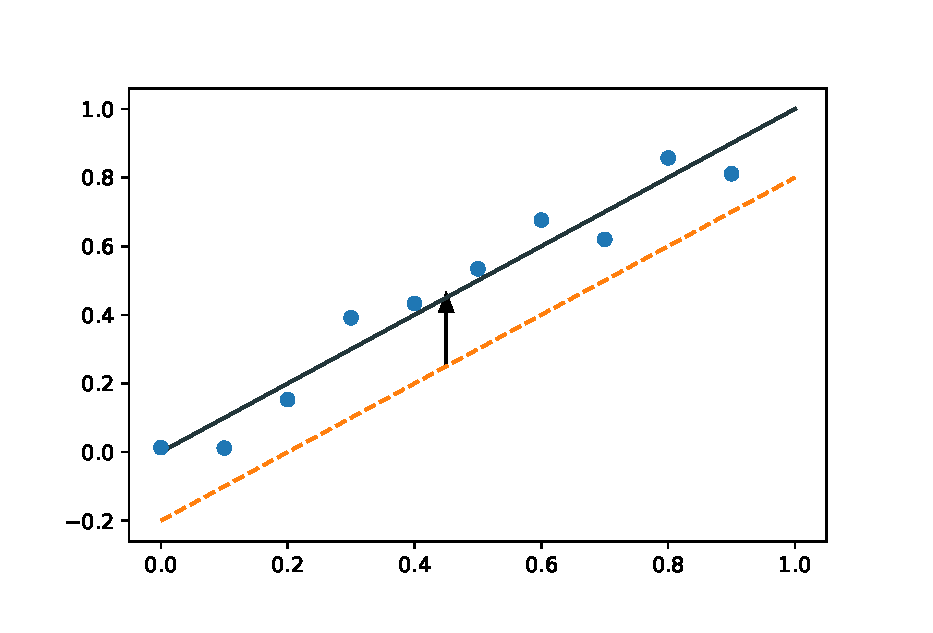
\includegraphics[width=5cm]{fig/arrange_params.eps}
      \caption{{\mgfamily 一次関数のモデルのパラメタ調整}}
    \end{figure}
  \end{columns}
\end{frame}
\section{Classification}
\begin{frame}{分類}
  クラスに分類された既存データを元に新規データを分類する
  \begin{table}
    \caption{{\mgfamily アルゴリズムとパラメタの決め方}}
    \begin{tabular}{@{} ll @{}}
      \toprule
      アルゴリズム &パラメタの決め方\\
      \midrule
      パーセプトロン & 確率的勾配降下法\\
      ロジスティク回帰 & 最尤推定法\\
      \bottomrule
    \end{tabular}
  \end{table}
\end{frame}
\section{Perceptron}
\begin{frame}{パーセプトロン, モデル}
  線形なモデル$f$を設定する
  \begin{columns}[T,onlytextwidth]
    \column{0.50\textwidth}
    \[f(x,y)=w_0+w_1x+w_2y\]
    \[f(x,y)>0\Rightarrow t = +1\]
    \[f(x,y)<0\Rightarrow t = -1\]
    \column{0.50\textwidth}
    \begin{figure}
      \centering
      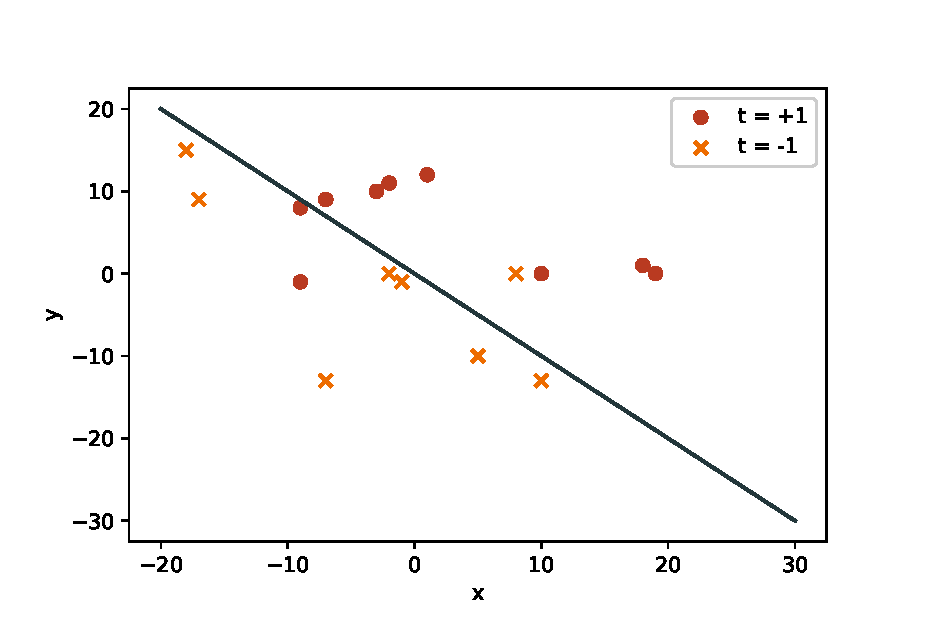
\includegraphics[width=5cm]{fig/scatter.eps}
      \caption{{\mgfamily 属性値$t=\pm1$をもつデータ群}}
    \end{figure}
  \end{columns}
  直線上の点$(x',y')$は$f(x',y')=0$をみたす
\end{frame}
\begin{frame}{パーセプトロン, 評価基準}
  誤分類の度合$E$が最小になる$w_i$を求める
  \begin{columns}[T,onlytextwidth]
    \column{0.50\textwidth}
    \begin{align*}
      E
      &=\sum_{i=1}^{N}{\left\{-\left(w_0+w_1x+w_2y\right)t_i\right\}}\\
      &=\sum_{i=1}^{N}{\left(-f(x_i,y_i)t_i\right)}
    \end{align*}
    \begin{itemize}
    \item $N$はデータ数
    \item 誤分類だと$-f(x_i,y_i)t_i>0$
    \end{itemize}
    \column{0.50\textwidth}
    \begin{figure}
      \centering
      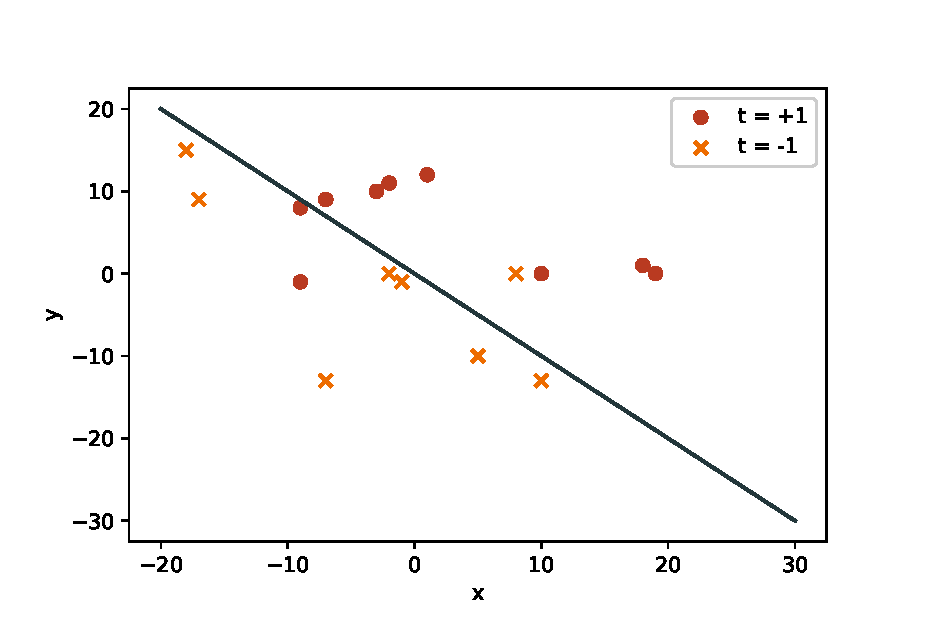
\includegraphics[width=5cm]{fig/scatter.eps}
      \caption{{\mgfamily 属性値$t=\pm1$をもつデータ群}}
    \end{figure}
  \end{columns}
\end{frame}
\begin{frame}{ロジスティック回帰, モデル}
  パーセプトロンと同じく線形モデル$f$を設定する
  \begin{columns}[T,onlytextwidth]
    \column{0.50\textwidth}
    \[f(x,y)=w_0+w_1x+w_2y\]
    \[f(x,y)>0\Rightarrow t = +1\]
    \[f(x,y)<0\Rightarrow t = -1\]
    \column{0.50\textwidth}
    \begin{figure}
      \centering
      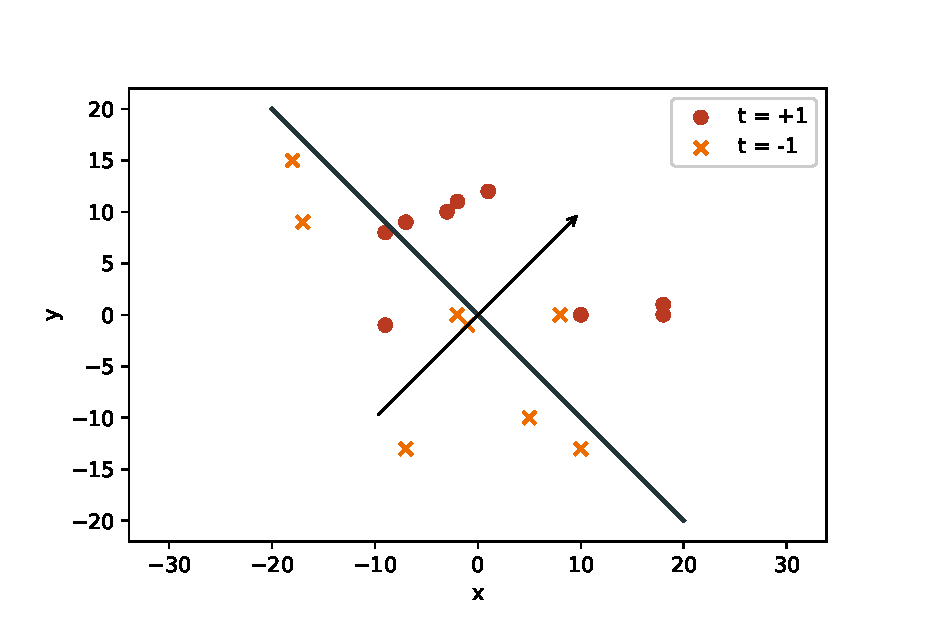
\includegraphics[width=5cm]{fig/direction.eps}
      \caption{$f(x,y)${\mgfamily が増加する向き}}
    \end{figure}
  \end{columns}
\end{frame}
\begin{frame}{ロジスティック回帰, モデル}
  ただし,$|f|$が大きいほど$t$である確率が高いとする
  \begin{columns}[T,onlytextwidth]
    \column{0.50\textwidth}
    ロジスティック関数
    \[\sigma\left(\alpha\right)=\frac{1}{1+e^{-\alpha}}\]
    を導入し,\\
    $(x',y')$が$t=1$である確率を\\
    \[0 < \sigma \left(f\left(x',y'\right)\right) < 1\]
    とする
    \column{0.50\textwidth}
    \begin{figure}
      \centering
      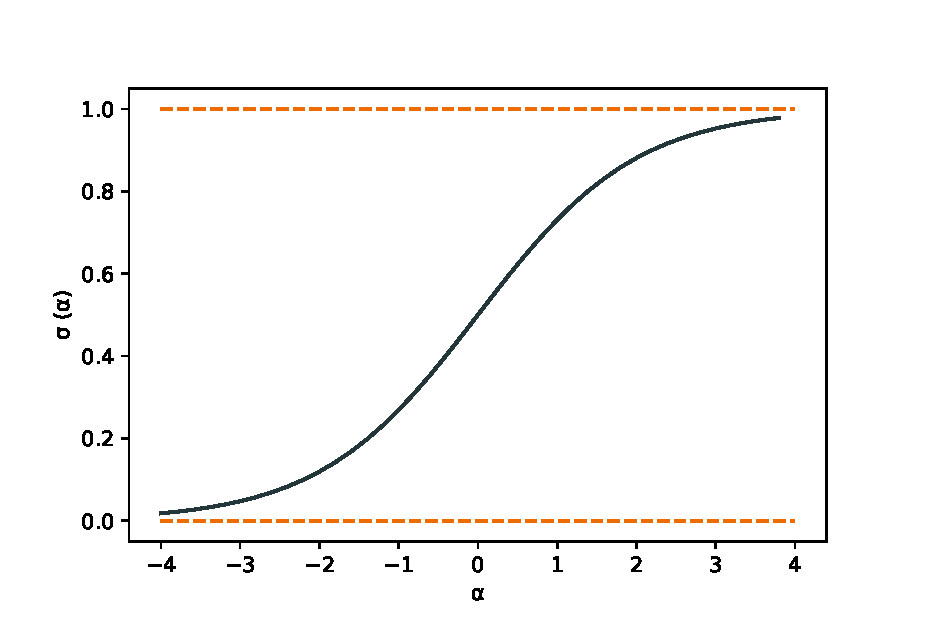
\includegraphics[width=5cm]{fig/sigmoid.eps}
      \caption{{\mgfamily ロジスティック関数のグラフ}}
    \end{figure}
  \end{columns}
\end{frame}
\begin{frame}{ロジスティック回帰, 評価基準}
  訓練データが得られる確率$P$を最大にする$w_i$を求める

  \begin{align*}
    p(x,y)&=\sigma(x_0+w_1x+w_2y)\\
    P&=\prod_{i}^{N}{p\left(x_i,y_i\right)}^{t_n}{\left\{1-p\left(x_i,y_i\right)\right\}}^{1-t_n}
  \end{align*}  
  訓練データは最も発生確率が高いデータであると仮定している
\end{frame}
\section{Regression}
\begin{frame}{回帰分析, モデル}
  データが$M$次多項式$f$に従うとする
\end{frame}
\begin{frame}{回帰分析, モデル}
  ただし,$x_n$の観測値$t$は正規分布に従い$f(x_n)\pm\sigma$に散らばる  
\end{frame}
\begin{frame}{回帰分析, 評価基準}
  訓練データの集合が生じる確率$P$を最大にするパラメタを求める
\end{frame}
\part{Unsupervised Learning}
\section{k-means clustering}
\begin{frame}{k平均法}
  データ間の距離を求め,データをk個のクラスタに分ける
\end{frame}
\begin{frame}{k平均法の適用例}
  ピクセルの色を似ている代表色に置き換えて減色する
\end{frame}
\end{document}
